\section{Vector Space Retrieval Model: TF Transformation}


\subsection{Ranking Function with TF-IDF Weighting}

\begin{equation*}
f(q, d) = \sum_{i=1}^N x_i y_i = \sum_{w \in q \cap d} c(w, q) c(w, d) \log \frac{M+1}{df(w)}
\end{equation*}

\begin{itemize}
\item $w \in q \cap d$ - all matched query (q) words in document (d)
\item $c(w, q)$ - count of word w in document d
\item $M$ - total number of documents in collection
\item $df(w)$ - Doc Frequency (total number of documents containing word w)
\end{itemize}

%\begin{figure}[H]
%    \centering
%    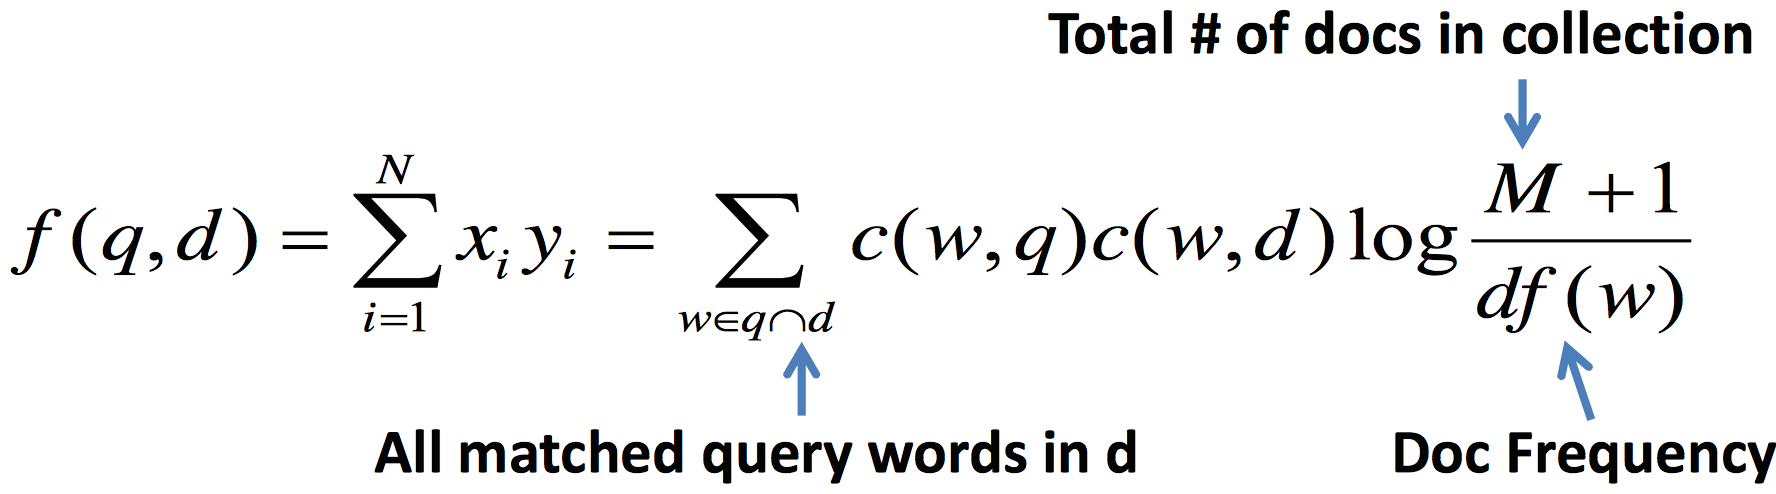
\includegraphics[width=\linewidth]{TF_IDF.png}
%\end{figure}



\subsection{TF Transformation: BM25 Transformation}
BM = Best Matching

\begin{figure}[H]
    \centering
    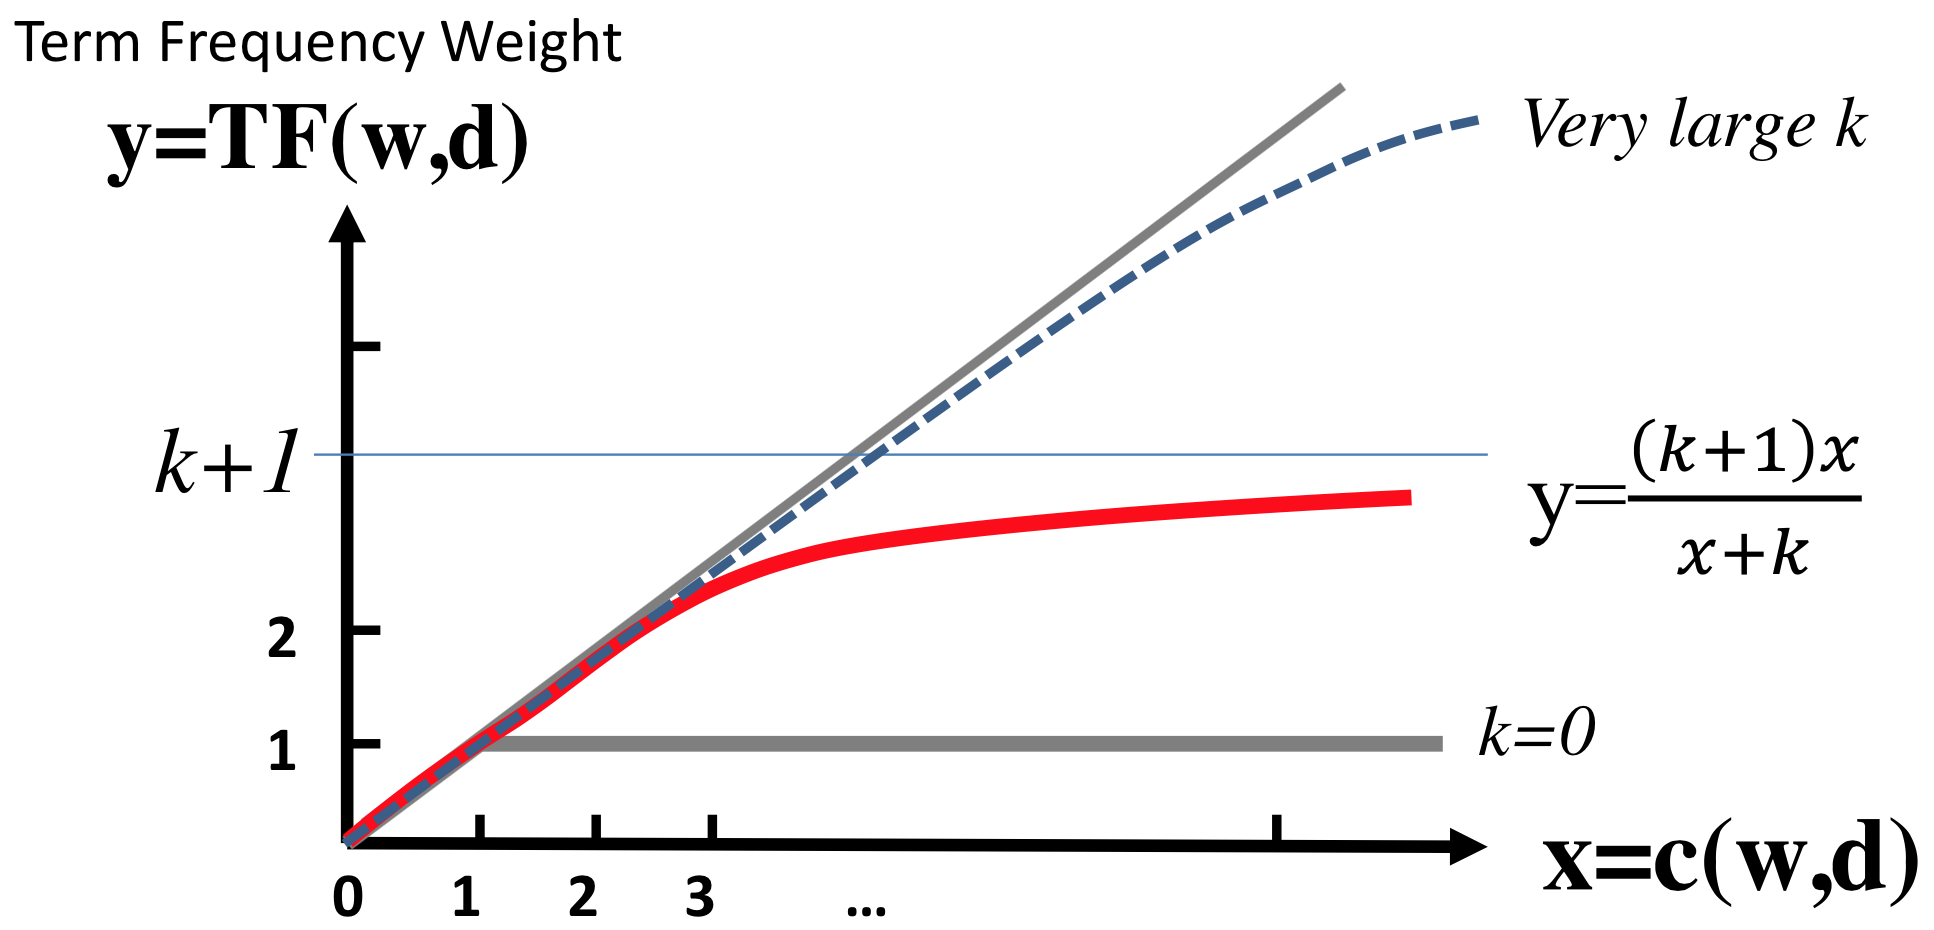
\includegraphics[width=0.75\linewidth]{BM25_transformation.png}
\end{figure}




\subsection{Summary}
\begin{itemize}
\item Sublinear TF Transformation is needed to
\begin{itemize}
\item capture the intuition of <<diminishing return>> from higher TF 
\item avoid dominance by one single term over all others
\end{itemize}

\item BM25 Transformation 
\begin{itemize}
\item has an upper bound
\item is robust and effective
\end{itemize}

\item Ranking function with BM25 TF ($k >= 0$):
\end{itemize}

\begin{equation*}
f(q, d) = \sum_{i=1}^N x_i y_i = \sum_{w \in q \cap d} c(w, q) \frac{(k+1) c(w, d)}{c(w, d) + k} \log \frac{M+1}{df(w)}
\end{equation*}